\documentclass[../main.tex]{subfiles}

\begin{document}
\section{Theory} \label{sec:theory}
\subsection{Wavefunction of Helium} \label{sec:QMProb}.
The single-particle wave function of an electron $i$ in the $1s$ state is given in terms of a dimensionless variable (the wave function is not normalized)

\[\vec{r}_i = x_i \vec{e}_x + y_i \vec{e}_y + z_i \vec{e}_z\]
as
\[\psi_{1s}(\vec{r}_i) = e^{-\alpha r_i}\]
Where $\alpha$ is a parameter set to 2, due to the two electrons, and the length $r_i$ is defined by
\[r_i = \sqrt{x_i^2 + y_i^2 + z_i^2}\]

For our system with two electrons, we have the product of the two $1s$ wave functions defined as
\[\Psi(\vec{r}_1, \vec{r}_2) = e^{-\alpha(r_1 + r_2)}\]

This leads to the integral (\ref{eq:int-to-solve}), which will be solved nummericaly with the three different methods mentioned earlier.
The value of the integral corresponds to the energy between the two electrons repelling each other due to Columb interactions.

\begin{equation}
  \langle \frac{1}{|\vec{r}_1 - \vec{r}_2|} \rangle = \int_{\infty}^\infty d\vec{r}_1 d\vec{r}_2 e^{-2\alpha(r_1 + r_2)} \frac{1}{\vec{r}_1 - \vec{r}_2}
  \label{eq:int-to-solve}
\end{equation}

\vspace{1cm}The analytical result is $5\pi/16^2$.

\subsection{Gaussian Quadrature} \label{sec:GQ}
The main idea of Gaussian quadrature is to integrate over a set of points $x_i$ not equally spaced with weights $w_i$, which are calculated in  the program Gauleg.cpp and Gauss Legendre.cpp). The weights are found throug ortogonal polynomials(Laguerre and Legendre polynomials) in a set interval. The points $x_i$ are chosen in a optimal sense and lie in the interval.

The intgral is approximated as
\[\int_a^b W(x)f(x) \approx \sum_{i=1}^n \omega_i f(x_i) \]

For a more detalied derivation and explenation?? of Gaussian qudrature see (Hjort-Jensen, 2015)


\subsubsection{Gauss-Legendre}\label{sec:GLQ}
Using Gauss-Legendre quadrature with Legendre polynomials will make it possible to utilize the integral numerically. The first step is to change the integration limits from  $-\infty$ and $\infty$ to $-\lambda$ and $\lambda$. The $\lambda$'s are found by inserting it for $r_i$ in the expression $e^{-\alpha r_i}$ because $r_i \approx \lambda$ when $e^{-\alpha r_i} \approx 0$. As we see from figure \ref{fig:expfunc}, $\lambda \in [-5,5]$ is therefore a good approximation for the integration limits.

\begin{figure}
  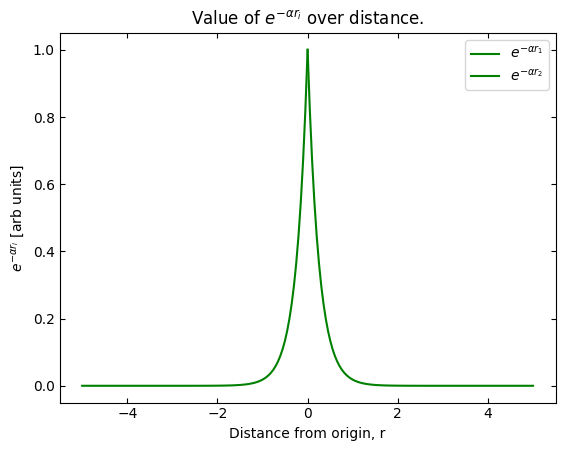
\includegraphics[width=\textwidth]{../img/expfunc_plot.png}
  \caption{Plot of wavefunction in one dimension}
  \label{fig:expfunc}
\end{figure}

Furthermore, the  weights and mesh points are computed using "gauleg"(see program exampleprog.cpp????).

Eventually ending up with a sixdimensional integral, where all six integration limits are the same.

\[\int_a^b\int_a^b\int_a^b\int_a^b\int_a^b\int_a^b e^{-x}f(x)dx \approx \sum_{i=1}^n w_i f(x_i)\]

\subsubsection{Improved Gauss-Quadrature- Laguerre} \label{sec:improved_GQ}
Gauss-Legendre quadrature gets the job done, but it is unstable and unsatisfactory. By changing to spherical coordinates and  replacing Legendre- with Laguerre polynomials an improvement in accuracy is expected. The Laguerre polynomials are defined for  $x \in [0, \infty)$,and in spherical coordinates:
\\

\[ d\vec{r}_1 d\vec{r}_2 = r_1^2 dr_1 r_2^2 dr_2 dcos(\theta_1) dcos(\theta_2) d\phi_1 d\phi_2\]
\\
with

\[\frac{1}{r_{12}} = \frac{1}{\sqrt{r_1^2 + r_2^2 - 2r_1r_2cos(\beta)}} \]
\\and


\[cos(\beta) = cos(\theta_1)cos(\theta_2) + sin(\theta_1)sin(\theta_2)cos(\phi_1 - \phi_2)\]
\\

For numerical integration, the deployment of the following relation is nessecary:

\[\int_0^\infty e^{-x}f(x)dx \approx \sum_{i=1}^n w_i f(x_i)\]
where $x_i$ is the $i$-th root of the Laguerre polynomial $L_n(x)$ and the weight $w_i$ is given by
\\
\[w_i = \frac{x_i}{(n+1)^2 [L_{n+1}(x_i)]^2}\]
\\
The Laguerre polynomials are defined by Rodrigues formula:
\[L_n(x) = \frac{e^x}{n!}\frac{d^n}{dx^n}\left(e^{-x} x^n\right) = \frac{1}{n!}\left(\frac{d}{dx}-1\right)^n x^n\]
or recursively relations:
\begin{align*}
  L_0(x) &= 1\\
  L_1(x) &= 1 - x\\
  L_{n+1}(x) &= \frac{(2n + 1 - x)L_n(x) - nL_{n-1}(x)}{n+1}\\
\end{align*}
\ref{sec:GLQ}


\subsection{Monte Carlo}
\subsubsection{Generalized}
\label{sec:MC}
Monte Carlo integration is based on the idea of finding the mean of a function in a domain by sampling random function values. This mean multiplied by the volume of the domain will be an approximation of the integral. \\

Say we have an integral $I$ of $f(\mathbf x)$ we want to find:

\begin{equation*}
  I=\int_D f(\mathbf x)d\mathbf x
\end{equation*}

where $\mathbf{x}$ is in the domain $D$. This integral can be approximated by using random numbers distributed on $D$ by the probability distribution function (PDF) $p(\mathbf x)$. Discretizing, the approximated integral now becomes

\begin{equation}
  I \approx \langle I \rangle = \frac{1}{N}\sum_{i=0}^N\frac{f(\mathbf x_i)}{p(\mathbf x_i)},
  \label{eq:genapproxMC}
\end{equation}

where  $N$ is the number of sampled values.

\subsubsection{Naïve approach (uniform PDF)}
To solve our six-dimensional integral, we first take the naïve approach and distribute our randomly chosen variables on the uniform distribution

\begin{equation*}
  \theta (x) = \bigg\{ \begin{matrix}\frac{1}{b-a}, & \text{for}\ x\in[a,b] \\ 0 & \text{else}\end{matrix},
\end{equation*}

and keep our variables $\mathbf r_1$ and $\mathbf r_2$ in cartesian coordinates. Putting the uniform distribution into (\ref{eq:genapproxMC}), we get the naïve approximation of an integral:

\begin{equation}
  \langle I\rangle = \frac{V}{N}\sum_{i=0}^Nf(\mathbf x_i).
\end{equation}

Here $V$ is the integration volume (for $d$ dimensions in cartesian coordinates $V=(b-a)^d$, with $b$ and $a$ being the integration limits for each dimension). Going back to our original integral (\ref{eq:int-to-solve}), our approximation of it using this method is

\end{document}
